\begin{ledgroupsized}[r]{120mm}
\footnotesize
\pstart
\noindent\textbf{Überlieferung:}
\pend
\end{ledgroupsized}
\begin{ledgroupsized}[r]{114mm}
\footnotesize
\pstart
\parindent -6mm 
\makebox[6mm][l]{\textit{L}}%
Konzept:
LH~XXXV~5,~28~Bl.~8\textendash9.
Ein Bogen~8\textsuperscript{o}.
Ränder beschnitten.
Drei Seiten.
Bl.~9~v\textsuperscript{o} leer.
\pend
\end{ledgroupsized}%
\selectlanguage{latin}
\vspace{8mm}
\pstart%
\noindent%
\href{\Scan{LH_35_05_28_008r}}%
{\lbrack8~r\textsuperscript{o}\rbrack} 
\edtext{Objectio viri\indexN{\textls{Vanni}, Giovanni Francesco 1638\textendash1709}
ut apparet peringeniosi contra receptissimum Staticorum\indexS{Statici} 
Theorema\indexS{Theorema Staticorum receptissimum} 
de momento gravis super plano inclinato\indexS{momentum gravis super plano inclinato},}{%
\lemma{Objectio \lbrack...\rbrack\ inclinato}%
\Cfootnote{\textsc{G.\,F. Vanni},\indexN{\textls{Vanni}, Giovanni Francesco 1638\textendash1709} \cite{01995}\textit{Specimen libri de momentis gravium etc. Autore I.\,F.\,V. Lucensi}, \cite{01023}\textit{AE} November 1684, S.\;511\textendash513. 
Vanni kritisiert
\indexN{\textls{Galilei} (Galilaeus, Galileus), Galileo 1564\textendash1642}%
\textsc{G.~Galilei}, %
\cite{00050}\textit{Discorsi}, %
Giornata Terza, De motu naturaliter accelerato; \glqq Aggiunta postuma dell'Autore\grqq\ %
nach dem Scholion zum 2.~Theorem (der Zusatz erschien erst in der posthumen Werkausgabe: \cite{01084}\textit{Opere}, Bologna 1656, Bd.~II, S.\;132\lbrack ter\rbrack\textendash134; \cite{00048}\textit{GO} VIII, S.\;216\textendash219 im Apparat) %
und
\indexN{\textls{Torricelli} (Torricellius), Evangelista 1608\textendash1647}%
\textsc{E.~Torricelli}, \textit{De motu gravium}, lib.~I
(\cite{00304}\textit{Opera geometrica}, Florenz 1644, S.\;99;
\cite{00108}\textit{TO}~II, S.\;105).}}
solvi omnino potest;
meretur tamen non contemni, quia ita speciosa est
ut negotium aliis quoque facessere possit. 
\pend
\begin{edfigure}%
\includegraphics[scale=1]{%
gesamttex/edit_VIII-4/images/LH_35_05_28_008-009_d1.pdf}
\edcaption{%
\edtext{\lbrack\textit{Fig.~1, erg. Hrsg. nach Vanni\indexN{\textls{Vanni}, Giovanni Francesco 1638\textendash1709}}\rbrack}{%
\lemma{\lbrack\textit{Fig.~1}\rbrack}%
\Cfootnote[nonum]{%
\cite{01995}a.\,a.\,O., S.\;512.}}}
\end{edfigure}
\pstart
Retenta
ejus figura, argumenti vis breviter huc redit: Gravis \textit{I}
momentum super plano inclinato\indexS{momentum gravis super plano inclinato} \textit{XC} est ad momentum
gravis absolutum seu perpendiculare\indexS{momentum gravis absolutum seu perpendiculare} ut \textit{XN} ad
\textit{XC}, per theorema receptum.\indexS{theorema Staticorum receptum} Et eodem modo,
ejusdem gravis momentum super plano inclinato\indexS{momentum gravis super plano inclinato} \textit{ZC}
erit ad idem momentum absolutum\indexS{momentum gravis absolutum} ut \textit{ZO} ad \textit{ZC}
seu ad \textit{XC}, quia \textit{ZC} et \textit{XC} ponuntur aequales.
Ergo summa horum duorum momentorum in planis
inclinatis\indexS{planum inclinatum} sustentantibus est ad momentum
absolutum\indexS{momentum absolutum} ut $XN+ZO$ ad \textit{XC}. Hactenus
recte. Jam vero summa haec aequatur momento
absoluto ut ait autor\indexN{\textls{Vanni}, Giovanni Francesco 1638\textendash1709}. Ergo $XN+ZO$ aequatur
ipsi \textit{XC} quod est absurdum. Verum
sciendum est causam falsae conclusionis non latere
in theoremate recepto,\indexS{theorema Staticorum receptum} sed in assumto \indexN{\textls{Vanni}, Giovanni Francesco 1638\textendash1709}viri docti,
quod nempe duo momenta in planis inclinatis\indexS{planum inclinatum sustentans}
sustentantibus simul sumta aequentur momento
absoluto.\indexS{momentum absolutum} Id quod illi
\edtext{nulla demonstratio,}{\lemma{}\Bfootnote{nulla \bars{nulla \textit{gestr.}} demonstratio,~\textit{L}}} 
sed probabilis consideratio persuaserat; et fraudi fuisse
videtur, quod illa vocavit partialia,\indexS{momentum partiale} hoc totale.\indexS{momentum totale}
Cum tamen componantur inter se partialia illa
non conjunctive\indexS{compositio momentorum conjunctiva seu cumulativa} 
seu cumulative ut ita dicam\lbrack,\rbrack\
sed disjunctive,\indexS{compositio momentorum disjunctiva} quia si conatus in uno plano
\href{\Scan{LH_35_05_28_008v}}%
{\lbrack8~v\textsuperscript{o}\rbrack} descendendi\indexS{conatus descendendi in plano} 
exitum sortietur, cessabit conatus
in altero. Praeterea (ne dicam nullum facile
repertum iri qui simili argumentatione sit
usus) certe multa falsa hoc modo possent
concludi. Imo quaecunque assignetur regula
pro planis inclinatis\indexS{planum inclinatum} ex ea tali modo argumentandi
absurdum deducam. Et poterit
grave millies millenis planis simul
\edtext{inniti. Imo}{\lemma{inniti}\Bfootnote{%
\textit{(1)}~, imo %
\textit{(2)}~. Imo~\textit{L}}}
infinitis, si sit in superficie concava
alicujus coni excavati apicem deorsum
vertentis; ubi infinitis suis punctis globus
superficiem conicam tangit,
\edtext{et plano conum}{\lemma{et}\Bfootnote{%
\textit{(1)}~cono planum %
\textit{(2)}~plano conum~\textit{L}}}
ibidem tangenti quolibet suo puncto inniti
putandus est.
\pend 
\begin{edfigure}[1em][1em]    	%
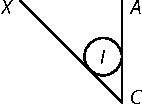
\includegraphics[scale=1]{
gesamttex/edit_VIII-4/images/LH_35_05_28_008-009_d2_008v.pdf}
\edcaption{\lbrack\textit{Fig.~2}\rbrack}
\end{edfigure}
\pstart
Et quid si grave inter
duo plana sit comprehensum\indexS{grave duobus planis innitens}
iisque innitatur, quorum
unum \textit{XC} sit
\edtext{inclinatum ad horizontem,\indexS{planum inclinatum}}{\lemma{inclinatum}\Bfootnote{%
\textit{(1)}~horizonti, %
\textit{(2)}~ad horizontem,~\textit{L}}} 
\textit{AC} alterum verticale?\indexS{planum verticale}
Utique si momenta respectiva
in duobus planis exercita
in unum addita\indexS{additio momentorum} aequantur
momento perpendiculari seu absoluto,\indexS{momentum perpendiculare seu absolutum} aequabuntur
ambo simul ipsorum uni nempe momento
in plano \textit{AC}, pars toti. Sed non est cur
his insistamus. Nam Theorema receptum
omnino apud Staticos\indexS{Statici}\indexS{Theorema apud Staticos receptum} habetur demonstratum,
\href{\Scan{LH_35_05_28_009r}}%
{\lbrack9~r\textsuperscript{o}\rbrack} nec meum est aliorum demonstrationes
repetere, quibus non puto resisti posse,
nisi quis principia statica,\indexS{principia statica} de centro
gravitatis et reciproca\indexS{principium de reciproca distantia aequiponderantium}
ab eo aequiponderantium\indexS{aequiponderantia}
distantia\lbrack,\rbrack\ evertere velit,
cui satisfacere hujus loci non est. Idem
fere dicendum arbitror de \edlabel{35_05_28_8-9_1a}%
\edtext{}{%
\xxref{35_05_28_8-9_1a}{35_05_28_8-9_1b}%
\lemma{docti cujusdam \lbrack...\rbrack\ oscillantium ascensu}%
\Cfootnote{Mit dem Ausdruck \glqq Mathematici Parisini\grqq\ ist 
der Abbé \indexN{\textls{Catelan}, François, Abbé de gest. nach 1719}Catelan gemeint. 
Dessen Kritik an \indexN{\textls{Huygens} (Hugenius, Ugenius, Hugens, Huguens), Christiaan 1629\textendash1695}Huygens' Satz über den Schwingungsmittelpunkt eines zusammengesetzten Pendels 
(\indexN{\textls{Huygens} (Hugenius, Ugenius, Hugens, Huguens), Christiaan 1629\textendash1695}\textsc{C.~Huygens}, \cite{00123}\textit{Horologium Oscillatorium}, 
pars IV, prop. IV, Paris 1673, S.\;98; \cite{00113}\textit{HO} XVIII, S.\;255) 
entfachte einen Streit, an dem sich neben 
\indexN{\textls{Catelan}, François, Abbé de gest. nach 1719}Catelan und 
\indexN{\textls{Huygens} (Hugenius, Ugenius, Hugens, Huguens), Christiaan 1629\textendash1695}Huygens auch 
\indexN{\textls{Bernoulli}, Jacob 1655\textendash1705}Jacob Bernoulli beteiligte. 
Die Beiträge erschienen zwischen Dezember 1681 und September 1684 im \cite{00157}\textit{Journal des Sçavans} und den \cite{02002}\textit{Nouvelles de la République des Lettres}.
Die \cite{01023}\textit{Acta Eruditorum} von September 1684 (S.\;416\textendash419) brachten einen anonymen (von \indexN{\textls{Lehmann}, Georg Heinrich fl. 1675\textendash1690}Georg Heinrich Lehmann verfassten) Bericht über die Geschehnisse bis Juli 1684: \textit{Relatio de controversia, quae hactenus inter Dn.\,Hugenium et Dn.\,Catelanum agitatur de centro Oscillationis, collecta ex Ephemeridibus Gallicis}\cite{02004}. Dort wird \indexN{\textls{Catelan}, François, Abbé de gest. nach 1719}Catelan u.\,a. als \glqq Mathematicus Parisiensis\grqq\ bezeichnet.}}%
docti cujusdam Mathematici Parisini\indexN{\textls{Catelan}, François, Abbé de gest. nach 1719} 
objectione in
his ipsis \cite{01023}\textit{Actis} mense Septembri hujus anni editis p.~416 relata,
\edtext{contra celeberrimi}{\lemma{contra}\Bfootnote{%
\textit{(1)}~propositionem ab %
\textit{(2)}~celeberrimi~\textit{L}}} 
Hugenii\indexN{\textls{Huygens} (Hugenius, Ugenius, Hugens, Huguens), Christiaan 1629\textendash1695}
positionem de centri gravitatis corporum
oscillantium\indexS{centrum gravitatis corporum oscillantium} 
ascensu.\indexS{ascensus centri gravitatis corporum oscillantium} 
\edlabel{35_05_28_8-9_1b} Itaque hortandi
sunt viri eruditi, ut in promovendis
potius scientiis industriam suam
ostendant, nec quae a Geometris\indexS{Geometra} praeclaris
accurate constituta sunt sine diligenti
examine labefactare aggrediantur.
Quamquam interim objectiones
\edtext{quoque, quarum solutio}{\lemma{quoque,}\Bfootnote{%
\textit{(1)}~quae lucem aliam %
\textit{(2)}~quarum so %
\textit{(3)}~quarum solutio~\textit{L}}} lucem
aliquam afferre potest, si absit
contentionis studium, laudem suam
mereantur.
\pend
